% Appendices: unlimited length, reviewers not required to read them. Check the CFP/OpenReview
% instructions on whether they go in the same PDF or are uploaded separately.

\section{The Full Question Bank}
\label{app:questions}

The bank has three layers. The first is the released bank of 101 core questions plus an operator
plug-in (\S\ref{sec:workflow-questions}), organized by where a performance gap might be and meant
to be worked through in order, so that the scope, the bound, the harness, the host, and the routing
are settled before the kernel body is touched. The second is the list of questions the skill asks the
agent to put to itself at every iteration. The third is the set of question categories observed in
the human messages of the case study, with verbatim examples.

Every core entry satisfies five admission rules. It carries no answer: it names a class of
hypothesis or a quantity to measure, never a technique to apply. It is answerable by a measurement
with stock tools (the profiler, the disassembler, the assembler's resource report, clock counters,
the harness). It is phrased against a bound, a roofline or a per-tile cycle budget, never against a
reference implementation; the five questions that only make sense when another implementation is
available to measure form their own conditional group. It names an architecture only as a parameter, and must make sense
on Ampere, Hopper, and Blackwell alike. And it names no operator: the attention structure the case
study needed (paging, softmax, split-KV, grouped heads) lives in a plug-in that the template at the
end of this section describes.

Tags: \textbf{[G]} generic; \textbf{[A]}, \textbf{[H]}, \textbf{[B]} Ampere-, Hopper-, or
Blackwell-specific checklist. Provenance tags give where each question came from: \textsc{tr}, the
human messages and skill of our traces; \textsc{sb}, \textsc{ps}, and \textsc{mo}, three public
GEMM optimization worklogs on Ampere \cite{boehm2022cudammm}, Hopper \cite{shankhdhar2024h100}, and
Blackwell \cite{modular2025blackwell}; \textsc{fa3} and \textsc{fa4}, the FlashAttention-3 and -4
papers \cite{shah2024flashattention3,zadouri2026flashattention4}. The first bank, distilled from the
traces alone after the campaigns, had 48 entries of which 21 named the upstream kernel as the
comparison and 13 named attention structure; the released bank is the result of removing both, which
moved 11 entries into the plug-in, rewrote 27, kept 10, and added the rest from the public sources.
The 72 entries whose provenance is the public sources alone have not yet been exercised by our agent.

\subsection{Core Bank}

\paragraph{A. Scope and triage.}
\begin{enumerate}[nosep,leftmargin=*]
\item Which losing scenarios share a kernel body, and which only share a host launcher? [G, \textsc{tr}]
\item Do the losers form one regime (large, small, irregular extents, padded dimension) or a grab bag? [G, \textsc{tr}]
\item Which problem dimension does the gap grow with: the streamed one (feed), the tiled one (tiling, scheduling), or none (a fixed tax)? [G, \textsc{tr}]
\item Is the gap in kernel cycles at locked clocks, or only in wall-clock (host, just-in-time compile, launch)? [G, \textsc{tr}]
\item Of the gaps and fixes I am listing, which have I already tried in this campaign, and why did they fail? [G, \textsc{tr}]
\item What do the scenarios below the target have in common, grouped by cause rather than by shape? [G, \textsc{tr}]
\end{enumerate}

\paragraph{B. Bound and regime.}
\begin{enumerate}[nosep,leftmargin=*,resume]
\item From the minimum bytes and FLOPs for this shape, which bound should dominate, and does the measured time match it? [G, \textsc{sb}]
\item Am I memory-, compute-, latency-, or launch-bound on this scenario, and does the answer change across the suite? [G, \textsc{sb}, \textsc{ps}]
\item For my tile, what are the cycle counts per unit (MMA, special-function, FMA, shared memory, L2 and DRAM), and which is largest? [G, \textsc{fa4}]
\item What is this GPU's ratio of MMA to special-function throughput, and does my instruction mix exceed it? [G, \textsc{fa3}, \textsc{fa4}]
\item Is the peak I measure against the right one: locked clocks, the power state the benchmark runs at, this data type's MMA rate? [G, \textsc{ps}]
\item Does shared-memory traffic scale with the number of MMA instructions rather than with tile size, and is it the binder? [G, \textsc{fa4}]
\item Could a power or thermal limit, not the kernel, be the ceiling at this size? [G, \textsc{ps}]
\end{enumerate}

\paragraph{C. Harness and measurement.}
\begin{enumerate}[nosep,leftmargin=*,resume]
\item Is the win larger than the noise measured now on this GPU, not the noise of an earlier run? [G, \textsc{tr}]
\item Am I timing what I think I am timing: warm-ups, cache flush, the same input distribution and data type as the baseline, kernel-only versus end-to-end? [G, \textsc{sb}, \textsc{ps}]
\item Is any of my time outside the kernel: metadata builds, combine passes, device-to-host copies, counter resets, descriptor builds? [G, \textsc{tr}]
\item Does the result hold on production-shaped problems, not only on the square or power-of-two sizes I tuned on? [G, \textsc{mo}, \textsc{ps}]
\item Have I recorded clocks, power state, warm-up count, iteration count, and variance before claiming a fraction of peak? [G, \textsc{mo}]
\end{enumerate}

\paragraph{D. Host, launch, routing.}
\begin{enumerate}[nosep,leftmargin=*,resume]
\item Is there a synchronous device-to-host copy left on the losing route that another route already avoids? [G, \textsc{tr}]
\item Is work redone per call on the host (descriptors, gather maps, schedules) that could be built once and cached? [G, \textsc{tr}, \textsc{fa4}]
\item Are there clears of counters, partial buffers, or outputs that nothing reads, or that could be fused? [G, \textsc{tr}]
\item For small grids, is the gap launch and setup overhead, with kernel-only time already near the bound? [G, \textsc{tr}]
\item Is this shape on the kernel I think it is, or on an older path because a routing gate is stale? [G, \textsc{tr}]
\item Would forcing the intended kernel on this shape, where numerically safe, close the gap without touching the kernel? [G, \textsc{tr}]
\item Is a feature flag or shape parameter forcing a slow instantiation that deserves its own specialization? [G, \textsc{tr}, \textsc{sb}]
\item For single-tile or underfilled grids, would a smaller tile or a split along the reduction dimension fill the machine? [G, \textsc{tr}, \textsc{sb}]
\end{enumerate}

\paragraph{E. Memory hierarchy and data movement.}
\begin{enumerate}[nosep,leftmargin=*,resume]
\item What is the achieved global-memory throughput against peak, and does the profiler flag uncoalesced or sector-inefficient accesses? [G, \textsc{sb}]
\item Does the SASS show the widest loads and stores for every operand, or are some still 32-bit? [G, \textsc{sb}]
\item Where the compiler refuses to vectorize, can I prove alignment to it instead of unrolling by hand? [G, \textsc{sb}]
\item Are shared-memory bank conflicts reported for the exact access pattern the MMA reads, and does fixing them help end to end? [G, \textsc{sb}, \textsc{mo}]
\item What is the L2 hit rate, and which concurrently resident CTAs actually share input data? [G, \textsc{sb}, \textsc{ps}]
\item Do neighboring CTAs load identical tiles that one load could serve? [G, \textsc{ps}, \textsc{mo}]
\item Are outputs written coalesced and vectorized through shared memory, with streaming hints where they are never re-read? [G, \textsc{mo}, \textsc{ps}]
\item Would a contiguous version of the same math meet the bound? If so, the gap is in the indirect or gathered loads. [G, \textsc{tr}]
\item Do intermediates round-trip through shared or on-chip memory more than once between producers and consumers? [G, \textsc{tr}]
\item Before tuning the epilogue, have I confirmed that the main loop is no longer bandwidth-bound? [G, \textsc{mo}]
\end{enumerate}

\paragraph{F. Compute issue and instruction mix.}
\begin{enumerate}[nosep,leftmargin=*,resume]
\item What dominates the instruction mix, math or address arithmetic and loads, and what is the FLOPs-per-load ratio per thread? [G, \textsc{sb}]
\item Am I using the widest MMA shape the instruction set offers, and what does the wider one cost in registers and shared memory? [G, \textsc{ps}, \textsc{fa4}]
\item Does the compiler already do the caching, unrolling, or reordering I am about to hand-write? [G, \textsc{sb}]
\item Is the non-MMA work (exponentials, conversions, reductions, rescaling) executing concurrently with the MMAs, or serialized by waits? [G, \textsc{fa3}, \textsc{fa4}]
\item Did I confirm the intended overlap in the SASS or a timeline, rather than assuming source order survived the compiler? [G, \textsc{fa3}]
\item Can part of a bottlenecked unit's work be re-expressed on an idle unit, and what fraction balances them? [G, \textsc{fa4}]
\item Which per-iteration bookkeeping is only occasionally necessary, and can it be made conditional while staying warp-uniform? [G, \textsc{fa4}]
\item Am I doing per-element work (masking, bounds checks, predication) on tiles that are provably full or provably empty? [G, \textsc{tr}]
\item Do concurrent warps contend for the same slow unit at the same time, and should their critical sections be staggered? [G, \textsc{fa3}]
\item Are there type conversions or silent up-casts on the hot path? [G, \textsc{tr}]
\end{enumerate}

\paragraph{G. Occupancy, registers, shared memory.}
\begin{enumerate}[nosep,leftmargin=*,resume]
\item From registers, shared memory, and threads per block, what occupancy is achievable, and do the stall reasons say more would help? [G, \textsc{sb}]
\item Is the binding limit the per-thread register cap rather than the register file, suggesting splitting the work across more warps? [G, \textsc{ps}]
\item Does the assembler warn about serialized MMAs or spills, and do I see local-memory traffic in the SASS? [G, \textsc{ps}]
\item Per warp role, what is the register budget for inputs, outputs, and temporaries, and does the sum fit? [G, \textsc{fa4}]
\item Are registers reallocated from issue-only warps to compute warps, and is the split tuned? [G, \textsc{fa3}, \textsc{ps}]
\item Can partial results be stored or consumed early to shorten live ranges? [G, \textsc{fa4}]
\item Did I size the multistage buffer from the shared-memory budget or pick a stage count, and do stages and output buffers compete? [G, \textsc{mo}]
\item For dimensions that are not multiples of the MMA tile, am I on padded math, and is a native-width instantiation possible? [G, \textsc{tr}]
\item Does my thread-to-data mapping need cross-lane shuffles for reductions, or could another mapping remove them? [G, \textsc{fa4}]
\end{enumerate}

\paragraph{H. Asynchrony and pipelining.}
\begin{enumerate}[nosep,leftmargin=*,resume]
\item Measured in cycles, how long are the load, compute, and store phases per tile, and which is not overlapped? [G, \textsc{ps}]
\item Have I drawn the dependency chain of one iteration and found which link leaves a unit idle? [G, \textsc{mo}]
\item Are data movement, MMA issue, and the non-MMA math in separate warps, or does one warp do all three in sequence? [G, \textsc{fa3}, \textsc{mo}]
\item How many independent MMAs are in flight, and is that enough to cover the non-MMA latency on this architecture? [G, \textsc{fa4}]
\item Are asynchronous operations committed without immediate waits, with the wait placed just before the consumer? [G, \textsc{fa3}]
\item Is the multistage pipeline at full depth on the losers, or draining early on partial tiles? [G, \textsc{tr}]
\item Which true dependence serializes the inner loop, and would one extra buffer let iteration $j{+}1$ overlap iteration $j$? [G, \textsc{fa3}]
\item Is the store path overlapped with the next tile's compute, or a serial tail? [G, \textsc{mo}, \textsc{ps}]
\item How many synchronizations per tile does the barrier API cost, and is the primitive itself the overhead? [G, \textsc{ps}]
\item Is any asynchronous wait or barrier issued under a divergent predicate? [G, \textsc{tr}]
\item For a deeper pipeline I adopted or rejected, did I weigh its register cost against the forced tile-size reduction? [G, \textsc{fa3}]
\end{enumerate}

\paragraph{I. Scheduling and load balance.}
\begin{enumerate}[nosep,leftmargin=*,resume]
\item Does the tile count divide evenly into the SM count on the shapes that matter, or is there a tail wave? [G, \textsc{mo}, \textsc{ps}]
\item In what order are tiles assigned to SMs, and would grouping or a space-filling curve raise L2 reuse? [G, \textsc{ps}, \textsc{mo}]
\item Would a persistent kernel help, and does its tile order preserve the locality the hardware scheduler gave me? [G, \textsc{ps}]
\item Does the kernel pay launch, shared-memory, and barrier re-initialization per tile instead of per CTA lifetime? [G, \textsc{mo}]
\item Where variable extents or masks make tiles unequal, which tiles are the long tail, and are they issued first? [G, \textsc{fa4}]
\item For data-dependent work sizes, is the schedule computed once and cached? [G, \textsc{fa4}]
\item If work is split along the reduction dimension, is the split heuristic, the combine, or the partial-buffer traffic the cost? [G, \textsc{tr}]
\item Do contended global reductions run on dedicated warps, in an order that avoids stall chains? [G, \textsc{fa3}, \textsc{fa4}]
\end{enumerate}

\paragraph{J. Low-precision numerics.}
\begin{enumerate}[nosep,leftmargin=*,resume]
\item What operand layout does the low-precision MMA require, and where is the fix-up done and hidden? [G, \textsc{fa3}]
\item Is the quantization-scale granularity matched to my tile, so that scaling rides on existing multiplies? [G, \textsc{fa3}]
\item What precision does the downstream consumer need, and did I measure error after that rounding against a high-precision reference? [G, \textsc{fa4}]
\item For any approximation or skipped step, is there a final exact normalization that bounds the drift? [G, \textsc{fa4}]
\end{enumerate}

\paragraph{K. If another implementation of this operator is available to measure.}
\begin{enumerate}[nosep,leftmargin=*,resume]
\item Am I comparing against its steady-state binary, not a cold just-in-time compile or a first-call path? [G, \textsc{tr}]
\item Same buffers, data type, flags, and split count as its call? [G, \textsc{tr}]
\item Which of its kernels is dispatched for this shape, and does it use a trick (a split, a specialization) that I do not? [G, \textsc{sb}]
\item On the same scenario, how do its measured unit utilizations and stall reasons differ from mine, and which difference matches my gap? [G, \textsc{tr}]
\item Is it constrained by the same rules as I am? If so and it is faster, which of my claimed limits does its existence refute? [G, \textsc{tr}]
\end{enumerate}

\paragraph{L. Ampere-class checklist.}
\begin{enumerate}[nosep,leftmargin=*,resume]
\item Am I on tensor-core MMA with matrix-fragment loads from shared memory, or on scalar FMA? [A, \textsc{sb}, \textsc{ps}]
\item Is global-to-shared staging asynchronous and double-buffered at both the global-to-shared and shared-to-register levels? [A, \textsc{sb}]
\item Are block, warp, and thread tiles chosen by autotuning on this GPU, with the grid filtered for alignment constraints? [A, \textsc{sb}]
\item Did the bank-conflict fix pay for itself, or did the layout change cost more than the conflicts? [A, \textsc{sb}]
\end{enumerate}

\paragraph{M. Hopper checklist.}
\begin{enumerate}[nosep,leftmargin=*,resume]
\item Are the MMAs the asynchronous warpgroup kind, with accumulators in registers budgeted per warpgroup? [H, \textsc{ps}, \textsc{fa3}]
\item Are tile loads done by the dedicated copy engine with a swizzle that matches the MMA's shared-memory layout? [H, \textsc{ps}]
\item Do producer warps release registers to consumers, with the split tuned to the accumulator footprint? [H, \textsc{ps}, \textsc{fa3}]
\item Are neighboring CTAs in a cluster multicasting shared operands, and was the cluster size tuned? [H, \textsc{ps}]
\item Are the barriers raw memory barriers with manual phase tracking, or a higher-level API that adds synchronizations? [H, \textsc{ps}]
\item Is the epilogue staged through shared memory and stored asynchronously, and does that trade against pipeline depth? [H, \textsc{ps}]
\end{enumerate}

\paragraph{N. Blackwell checklist.}
\begin{enumerate}[nosep,leftmargin=*,resume]
\item Are the MMAs fully asynchronous into tensor memory, issued by one thread, with completion signaled through barriers rather than waits? [B, \textsc{mo}, \textsc{fa4}]
\item Is tensor memory allocated once per CTA lifetime, and could its columns be split so the next tile accumulates while the last drains? [B, \textsc{mo}]
\item Is the accumulator layout in tensor memory spilling or serializing the MMA against the consumer warps? [B, \textsc{tr}]
\item Would a two-SM MMA pair halve per-SM operand traffic and shared-memory footprint for this tile? [B, \textsc{mo}, \textsc{fa4}]
\item Is only the leader CTA issuing MMAs, with peer barriers arrived at cluster scope? [B, \textsc{mo}]
\item Is a static tile scheduler assuming all SMs are free where the hardware launch-control scheduler could rebalance, and is scheduler latency hidden under the next load? [B, \textsc{mo}]
\item Is tensor-memory-to-register traffic off the critical path, and which register-resident fix-ups can move to a separate warp? [B, \textsc{fa4}]
\item Given that the special-function unit did not scale with the MMA on this architecture, what fraction of that unit's work must move elsewhere? [B, \textsc{fa4}]
\end{enumerate}

\paragraph{O. Operator plug-in template.}
A plug-in supplies, for one operator, five things: its regimes; its irregular-work structure; its
non-MMA units; its reduction splits; and its indirect loads. Each has a generic ancestor in the core
(entries 2, 71, 40, 73, and 34 respectively), so the core already asks about it in the abstract and
the plug-in only names the instance. The attention plug-in used in the case study lists, as regimes,
prefill versus decode, dense versus paged key--value cache, short versus long context, and grouped
or multi-query heads; as irregular work, causal and sliding-window masks and variable lengths; as
non-MMA units, the softmax exponential and the online rescale; as reduction split, split-KV decode
and its combine; and as indirect loads, page-table gathers. Its eleven questions (whether grouped
and multi-query losers show the same relative gap as multi-head at equal tokens; whether the
softmax and correction of two stacked tile halves overlap or serialize; whether a paged loser is
still feed-latency-bound after the gather and preload fixes; whether contiguous loads on the same
math would meet the bound; whether the hardware gather or a coalesced asynchronous copy is the right
loader; whether short decodes pay gather and descriptor setup that does not amortize; whether the
gap tracks page fragmentation; whether the decoupled key and value rings are balanced on the
unequal-head-dimension path; whether softmax, rescale, and masking between MMAs burn issue slots
that specialized warps would hide; whether the split-KV heuristic, the combine, or the partial
buffers are the cost; and whether paged-to-contiguous on the same problem size closes the gap) are
the attention instances of core entries 2, 45, 34, 34, 34, 22, 34, 61, 40, 73, and 34.

\subsection{The Skill's ``Ask Yourself'' List}
The skill (\S\ref{sec:workflow-skill}) instructs the agent to ask itself the following at every
iteration:
\begin{enumerate}[nosep,leftmargin=*]
\item Which bound binds on this scenario (bandwidth, MMA, special-function unit, shared-memory bandwidth, issue slots, launch), and what fraction of it do we reach?
\item Is the gap in kernel cycles, or outside the kernel (host, launch, routing, harness)?
\item Which single unit or stage has the largest excess over its cycle budget, and what is my hypothesis for why?
\item Do the losing scenarios share one cause, and have I grouped them before fixing any?
\item Should the losing regime have its own kernel instead of a flag in a shared one?
\item Is every asynchronous mechanism this architecture offers actually asynchronous in my SASS, or are waits placed where they serialize?
\item Is the win I just measured larger than the noise of this GPU at this moment, and does it hold on the other regimes?
\item If another implementation of this operator can be measured on this machine, how do its profile and launch path differ from mine, and which difference explains my gap?
\end{enumerate}

\subsection{Categories Observed in the Human Messages}
Table~\ref{tab:qbank-human} lists the eight categories of \S\ref{sec:workflow-questions} with verbatim
examples from the traces and the outcome they led to where one is documented
(\S\ref{sec:eval-cases}). Counts are over the 162 human messages; a message is counted in a category
when its primary act was a question or a question-shaped correction of that kind. Eight further
questions concerned repository housekeeping and are omitted.

\begin{table*}[t]
\centering\small
\caption{Question categories in the human messages, with verbatim examples.}
\label{tab:qbank-human}
\setlength{\tabcolsep}{4pt}\footnotesize
\begin{tabular}{@{}p{0.17\textwidth}rp{0.56\textwidth}p{0.2\textwidth}@{}}
\toprule
Category & $n$ & Examples & Documented outcome \\
\midrule
Measurement check & 13 &
``are you sure these improvements are not just noise? you used the noise level from a previous run''; ``what is the overall performance compared to FA3? Wasn't it 0.96 before?''; ``are the values in the tables latencies or speedups?'' &
Re-measurement on an idle GPU; two claimed wins withdrawn. \\
\addlinespace
Bound differencing & 10 &
``isn't the original FA3 code constrained by the same harness rules as our implementation? Why can FA3 reach high performance and we can't?''; ``can you explain what you mean by `genuine ceilings within the harness rules'?'' &
Host-side fill found; split-KV 0.87 $\to$ 0.97, geomean 1.02 $\to$ 1.13. \\
\addlinespace
Benchmark validity & 7 &
``what shapes does FA3 use for testing?''; ``are the scenarios comprehensive compared with SOL-ExecBench?''; ``how do we do in non-GQA test cases?'' &
Suite 40 $\to$ 58 $\to$ 105 scenarios; two silent wrong outputs found. \\
\addlinespace
Gap triage & 7 &
``what configs are bringing down the geomean? which ones are lower than 0.8x the speed of FA3?''; ``what do the configs that are less than 0.95x of FA3 have in common? Please group the slow configs by issue'' &
Scalar fallback exposed; 0.44 $\to$ 0.96. \\
\addlinespace
Agent process & 6 &
``didn't you already try that before?''; ``of these gaps, which ones have we already tried and why did they fail?''; ``why are you establishing the baselines for 2h? this should only have taken a few minutes'' &
Earlier transcripts reviewed before the next rewrite. \\
\addlinespace
Challenge a limit & 5 &
``why do you think the goal was achieved? we're still significantly below 1.0x''; ``this is not a rare corner, don't be lazy. please keep going until you reach 1.0x parity'' &
Premature ``goal met'' retracted; fp8 hd256 0.20/0.34 $\to$ 0.66/0.77. \\
\addlinespace
Strategy options & 5 &
``ok, so what do you recommend to do now to close the gap?''; ``should we use specialized kernels for the scenarios where we are slower (decode vs.\ prefill, long vs.\ short context)?'' &
Per-regime kernel family adopted on Blackwell (\S\ref{sec:kernels}). \\
\addlinespace
Hypothesis check & 3 &
``is it ncu that hangs or our kernel?''; ``before trying that, please double check your hypothesis to ensure you are certain on the cause of the gap and the method to fix it'' &
Divergent \texttt{tcgen05.wait} found; 8 hangs fixed. \\
\bottomrule
\end{tabular}
\end{table*}

\section{Case-Study Kernel Details}
\label{app:kernels}

\begin{figure*}[t]
\centering
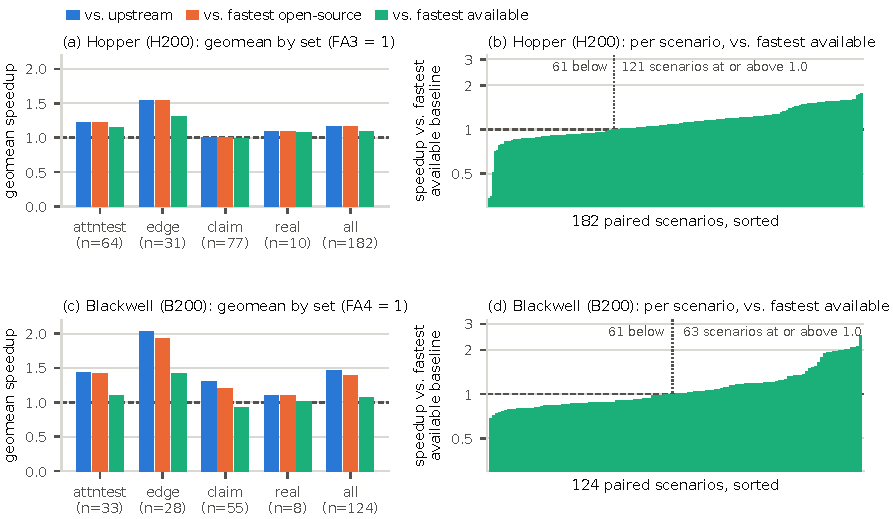
\includegraphics[width=\textwidth]{figures/casestudy.pdf}
\caption{Both kernels against three baselines. Left: geomean speedup per scenario set vs.\ the
upstream kernel, vs.\ the fastest open-source implementation per scenario (upstream or FlashInfer),
and vs.\ the fastest available implementation (also cuDNN). Right: every paired scenario sorted by
speedup over the fastest available baseline. On Hopper (top) the open-source and upstream columns
coincide because FlashInfer never beats FA3, and cuDNN is the fastest baseline on 54 of 182
scenarios; on Blackwell (bottom) cuDNN is the fastest baseline on 92 of 124, which is why the
headline shrinks more. The right tails are the \texttt{edge} sets, whose short kernels expose
upstream dispatch overhead.}
\label{fig:casestudy}
\end{figure*}
% Material moved out of Sec.~\ref{sec:kernels}. Numbers from the flash-cuda 2026-08 snapshot
% (README.md, docs/results_blackwell_*.csv, docs/blackwell_gap_analysis.md); re-measure before submission.

\subsection{\fathree}
The Hopper kernel is organized as a dispatcher over specialized paths, with the scalar seed retained
as the fallback for anything not yet specialized. The fast paths are warp-specialized: one producer
warpgroup issues TMA bulk-tensor loads of K and V into a
three-stage shared-memory ring ordered by mbarrier phases, while two consumer warpgroups run
asynchronous \texttt{wgmma} MMAs on a $128\times128$ CTA tile, with \texttt{setmaxnreg} moving
registers from the producer (40 per thread) to the consumers (up to 168). Prefill is persistent: Q
tiles arrive by TMA, a dynamic scheduler hands out tiles, and the two consumer warpgroups ping-pong so
that one warpgroup's softmax overlaps the other's MMAs. Masking is resolved per tile into a $[lo,hi)$
key range so that fully visible tiles skip the mask and fully masked tiles exit before the main loop.
Decode uses a separate kernel with split-KV and a combine pass, with split heuristics chosen per
shape. The fp8 path runs native e4m3 \texttt{wgmma}; for head dimension 64 it pads the Q and K tiles
to 128 columns so that the 128-byte swizzle stride composes and contracts only over the real columns,
which replaced an LSU-bound convert pass and took that scenario from 0.30$\times$ to 0.98$\times$.
Attention sinks are folded into the softmax denominator at the epilogue, \texttt{cache\_leftpad} is an
absolute lower bound on the key index with leading-tile pruning, and unequal head dimensions
(192/128) are handled by templating the two dimensions separately in prefill and decode.

\paragraph{The head-dimension-256 limit.} The output accumulator alone takes 128 registers per
consumer thread, which forces one CTA per SM and leaves the consumer starved on K/V arrival (NCU:
barrier and long-scoreboard bound, tensor pipe at 44\%). The hand-written 128-byte swizzle composes
only at key-tile widths of 48, 64, and 128; FA3 reaches its width of 80 because CUTLASS's register
allocator schedules that tile without serializing \texttt{wgmma}. A half-height Q tile with a deeper
ring (0.72$\times$: occupancy, not ring depth, is binding), a 240-register rebalance (deadlocks at the
65,536-register edge), and a head-dimension split (pays a 1.5$\times$ redundant QK cost) were each
measured and lost; the collective rewrite that followed brought the scenario to 0.94$\times$ in the
final measurement.

\paragraph{Per-set results.} The Hopper suite is the same 182 scenario definitions as Blackwell's,
all of which \fathree supports. Over the FA3 test grids (\texttt{attntest}, 64): 1.22$\times$, 54 at
or above parity, worst 0.89. Over the masking and boundary grid (\texttt{edge}, 31): 1.55$\times$,
30 at or above parity. Over the paper-style sweeps (\texttt{claim}, 77): 1.01$\times$, 44 at or above
parity, with the per-group geomeans ranging from 0.67 (dense fp8 prefill, 8 scenarios) through 0.87
(causal $d=256$), 0.92 (causal $d=128$), 0.96 (prefill) and 1.05 (chunked prefill) to 1.20 (decode up
to 4K), 1.22 (speculative decode) and 1.38 (ragged prefill). Over the production shapes
(\texttt{real}, 10): 1.10$\times$, 7 at or above parity. cuDNN 9.20 fused SDPA, fed the same packed
and paged buffers, supports 145 of the 182 and runs at 0.86$\times$ FA3 in geomean; \fathree is faster
on 111 of them, with cuDNN winning dense prefill by up to 1.6$\times$ and losing paged decode by up to
5.5$\times$. FlashInfer supports 32 and runs at 0.72$\times$ FA3; \fathree is faster on all 32. The
worst Hopper scenarios are dense fp8 prefill at $d=64$ and 8K context (0.34$\times$), a softcapped
4K prefill (0.51$\times$), $d=96$ (0.71$\times$), and a 4K sliding window (0.79$\times$).
Table~\ref{tab:per-scenario-hopper} lists every scenario.

\subsection{\fafour}
The Blackwell kernel is a family with configuration-aware routing on the host:
\begin{itemize}
\item \texttt{fwd\_kernel\_fa4}: a persistent warp-specialized collective
with a 256-row Q tile as two stacked 128-row halves sharing K and V, two
softmax warpgroups in an ordered ping-pong, a correction warpgroup rescaling O in tensor memory with
packed f32x2 math, one MMA warp, and load warps, in a 512-thread CTA with a 192/64/64 register plan,
longest-processing-time persistent scheduling, and continuous cross-tile overlap. Sliding windows,
attention sinks, padded head dimension 96, and paged KV are \texttt{if constexpr} template
parameters; the default instantiation is SASS-byte-identical to the ungrafted kernel.
\item \texttt{fwd\_kernel\_fa4dk}: the same for $d_{qk}=192, d_v=128$ with a decoupled K-depth-2,
V-depth-1 ring that fits the 227~KB shared-memory cap (0.21$\times$ to 1.06$\times$).
\item \texttt{fwd\_kernel\_fa4\_paged}: the same choreography on a paged gather. Pages aligned to
the 8-row swizzle atom load as TMA boxes (8 per tile instead of about 4,096 \texttt{cp.async}
issues); other page sizes use a warp-uniform \texttt{tile::gather4} loader (the divergent-lane
version had made TMA issue 29.5\% of all executed instructions); a run detector upgrades tiles whose
physical pages are consecutive to full-width boxes at run time.
\item \texttt{fwd\_kernel\_ws2} and the paged decode kernels for small, ragged, and decode shapes,
with split-KV and a combine pass.
\end{itemize}
Host-side design: no route performs a synchronous device-to-host copy (one
\texttt{cu\_seqlens.to(cpu)} cost about 38~$\mu$s per call and had hidden a kernel already faster
than upstream); the persistent scheduler's counter resets itself on device; large-query paged prefill
with page sizes the TMA box cannot express is materialized once into a contiguous cache (two passes
over the unique bytes, under 1\% of the attention's own traffic) and routed to the dense kernel; and
mixed batches are split by query length into two launches so that decode sequences read K/V once per
KV head.

\paragraph{Remaining known costs}, in order of measured size: a K/V ring of two pairs where the
shared-memory budget would admit two and a half; all \texttt{ex2} on the XU pipe, with no fraction
emulated on the FMA pipe; the correction warpgroup also running the epilogue rather than a separate
warp; page rows staged through shared memory rather than held in registers; and a software row-max
instead of the hardware reduction.

\paragraph{Scenario sets.} \texttt{attntest} (64): the FA3 grids ported to FA4. \texttt{edge} (31):
a dense $(s_q,s_k)$ masking and boundary grid from FA4's own tests. \texttt{claim} (77): causal and
non-causal sweeps over sequence length and head dimension in the style of the FA4 paper, plus
decode, chunked prefill, speculative, mixed-batch, and fp8-KV groups. \texttt{real} (10): GQA shapes
from SOL-ExecBench (Llama-3.1-8B, Qwen3-30B-A3B; decode and paged prefill; page size 1).

\paragraph{Caveats.} The Blackwell \texttt{edge} kernels take 50--100~$\mu$s under FA4, so its
2.0$\times$ is dominated by FA4's Python and CuteDSL dispatch; kernel-only ratios there are near
parity. The Hopper \texttt{edge} set (1.55$\times$) is in the same short-kernel regime against
FA3's compiled op and its scheduler-metadata call, and should be read with the same caution. The six
bf16-query/fp8-KV decode scenarios in \texttt{claim} run at 4.5--9.9$\times$ because FA4 is slow on
them; excluding them gives 1.37$\times$ vs.\ upstream, 1.32$\times$ vs.\ fastest open-source, and
1.08$\times$ vs.\ fastest available over the remaining 118. The run-detecting TMA path benefits from
the harness building page tables with \texttt{arange}; with it disabled, the two long-context decode
scenarios fall from 1.01 and 0.90 to 0.77 and 0.78$\times$. Noise is about $\pm$1.5\% for repeated
single-GPU runs and $\pm$5\% across four-GPU sweeps.

\paragraph{Where it loses, with causes.} Dense long context (0.88--0.92$\times$) executes exactly
FA4's tensor work (identical \texttt{tcgen05} op counts per block) over 33\% more cycles; the idle
tensor pipe is attributable to twice as many mbarrier waits per block (47.7 vs.\ 24.5), with memory,
occupancy, and the softmax transcendentals measured and ruled out. Batch-64 decode (0.88$\times$)
pays a cold start per CTA over 3.5 waves where FA4 runs a persistent grid. Head dimension 96
(0.85$\times$) runs on the padded 128-wide path. A mixed prefill/decode batch (0.78$\times$) is within
its historical noise band. Production shapes: short-context decode 1.50 and 1.49$\times$ FA4
(Llama-3.1-8B and Qwen3-30B at 512 tokens), long-context decode 1.17 and 1.01$\times$ (4K and 16K),
paged prefill 1.04, 0.98, and 0.91$\times$.

\section{Per-Scenario Results}
\label{app:per-scenario}
Tables~\ref{tab:per-scenario-hopper} and \ref{tab:per-scenario-blackwell} list every scenario of
both suites with the upstream latency and the speedup of each implementation over upstream. They are
generated from the released result files by \texttt{scripts/make\_appendix\_tables.py}; Hopper rows
are per-scenario medians over three repeats.

\onecolumn\footnotesize
\begin{longtable}{@{}llrrrrr@{}}
\caption{Per-scenario results on H200. Speedups are upstream (FA3) time over the implementation's time; ``best'' is our speedup over the fastest available baseline (upstream, cuDNN, or FlashInfer). ``---'': the implementation does not support the scenario.}\label{tab:per-scenario-hopper}\\
\toprule Set & Scenario & FA3 ($\mu$s) & ours & cuDNN & FlashInfer & best \\ \midrule \endfirsthead
\toprule Set & Scenario & FA3 ($\mu$s) & ours & cuDNN & FlashInfer & best \\ \midrule \endhead
\bottomrule \endfoot
attntest & attn\_dense\_hd64\_causal & 138.4 & 1.40 & 1.60 & --- & 0.88 \\
attntest & attn\_dense\_hd96\_causal & 168.7 & 1.07 & 1.49 & --- & 0.72 \\
attntest & attn\_dense\_hd128\_causal & 135.3 & 1.06 & 1.16 & --- & 0.91 \\
attntest & attn\_dense\_hd192\_causal & 171.2 & 0.97 & 1.12 & --- & 0.87 \\
attntest & attn\_dense\_hd256\_causal & 203.6 & 0.94 & 1.09 & --- & 0.87 \\
attntest & attn\_dense\_hd128\_noncausal & 178.7 & 1.05 & 1.18 & --- & 0.89 \\
attntest & attn\_dense\_hd128\_nc4k & 450.7 & 0.92 & 0.97 & --- & 0.92 \\
attntest & attn\_dense\_hd128\_gqa & 127.1 & 1.05 & 1.11 & --- & 0.94 \\
attntest & attn\_dense\_hd128\_mqa & 126.3 & 1.05 & 1.10 & --- & 0.95 \\
attntest & attn\_dense\_hd128\_fp16 & 134.1 & 1.05 & 1.15 & --- & 0.92 \\
attntest & attn\_dense\_hd128\_fp8 & 155.2 & 1.04 & --- & --- & 1.04 \\
attntest & attn\_dense\_hd128\_softcap & 147.7 & 1.01 & --- & --- & 1.01 \\
attntest & attn\_dense\_hd128\_local & 100.9 & 1.11 & 1.03 & --- & 1.08 \\
attntest & attn\_dense\_hd128\_oddseq & 43.5 & 1.40 & 1.33 & --- & 1.05 \\
attntest & attn\_dense\_hd128\_seq256 & 50.5 & 1.21 & 1.41 & --- & 0.85 \\
attntest & attn\_dense\_hd128\_large4k & 259.2 & 0.89 & 0.91 & --- & 0.89 \\
attntest & attn\_dense\_hd128\_splits3 & 151.9 & 1.26 & 1.35 & --- & 0.93 \\
attntest & attn\_varlen\_hd128\_causal & 37.6 & 1.55 & 0.96 & --- & 1.55 \\
attntest & attn\_varlen\_hd128\_noncausal & 36.9 & 1.54 & 0.94 & --- & 1.54 \\
attntest & attn\_varlen\_hd64\_causal & 38.4 & 1.77 & 1.02 & --- & 1.74 \\
attntest & attn\_varlen\_hd128\_mqa & 37.9 & 1.56 & 0.96 & --- & 1.56 \\
attntest & attn\_kv\_hd128\_decode\_mha & 59.7 & 1.26 & 0.54 & 0.67 & 1.26 \\
attntest & attn\_kv\_hd128\_decode\_gqa5 & 42.3 & 1.44 & 0.49 & 0.60 & 1.44 \\
attntest & attn\_kv\_hd128\_decode\_mqa32 & 41.0 & 1.60 & 0.95 & 0.57 & 1.60 \\
attntest & attn\_kv\_hd128\_decode\_qlen120 & 76.4 & 1.12 & 0.74 & --- & 1.12 \\
attntest & attn\_kv\_hd128\_decode\_qlen8 & 61.9 & 1.27 & 0.62 & --- & 1.27 \\
attntest & attn\_kv\_hd64\_decode\_gqa3 & 41.1 & 1.47 & 0.43 & 0.59 & 1.47 \\
attntest & attn\_kv\_hd256\_decode\_mqa16 & 46.5 & 1.35 & 0.18 & 0.53 & 1.35 \\
attntest & attn\_kv\_hd128\_decode\_noncausal & 41.0 & 1.41 & 1.29 & --- & 1.09 \\
attntest & attn\_kv\_hd128\_fp8\_decode & 51.5 & 1.14 & --- & --- & 1.14 \\
attntest & attn\_kv\_hd128\_split2 & 67.8 & 1.20 & 0.49 & 0.76 & 1.20 \\
attntest & attn\_kv\_hd256\_split\_auto & 54.9 & 1.40 & 0.20 & 0.55 & 1.40 \\
attntest & attn\_kv\_hd128\_local\_decode & 40.8 & 1.50 & 0.89 & --- & 1.50 \\
attntest & attn\_kv\_hd128\_decode\_gqa9 & 45.7 & 1.40 & 0.53 & 0.60 & 1.40 \\
attntest & attn\_kv\_hd128\_decode\_gqa7 & 52.8 & 1.32 & 0.48 & 0.66 & 1.32 \\
attntest & attn\_kv\_hd128\_decode\_128k\_splitkv & 526.6 & 1.02 & 0.20 & 0.77 & 1.02 \\
attntest & attn\_kv\_hd128\_page1 & 41.8 & 1.49 & 0.62 & --- & 1.49 \\
attntest & attn\_kv\_hd128\_page4 & 42.0 & 1.50 & 0.66 & --- & 1.50 \\
attntest & attn\_kv\_hd128\_page128 & 42.6 & 1.50 & 0.66 & 0.61 & 1.50 \\
attntest & attn\_kv\_hd128\_ctx20k & 72.4 & 1.18 & 0.20 & --- & 1.18 \\
attntest & attn\_kv\_hd128\_prefill3577 & 194.1 & 1.03 & 0.82 & --- & 1.03 \\
attntest & attn\_kv\_hd128\_dec339 & 35.5 & 1.35 & 1.18 & 0.53 & 1.15 \\
attntest & attn\_kv\_hd128\_dec1024 & 41.8 & 1.55 & 0.95 & --- & 1.55 \\
attntest & attn\_kv\_hd128\_dec800 & 46.0 & 1.38 & 1.09 & --- & 1.27 \\
attntest & attn\_dense\_hd192\_dv128 & 141.4 & 0.94 & 1.01 & --- & 0.93 \\
attntest & attn\_varlen\_hd192\_dv128 & 39.3 & 1.49 & 0.97 & --- & 1.49 \\
attntest & attn\_dense\_hd64\_fp16 & 137.0 & 1.39 & 1.60 & --- & 0.87 \\
attntest & attn\_dense\_hd192\_fp16 & 173.8 & 0.98 & 1.11 & --- & 0.88 \\
attntest & attn\_dense\_hd128\_fp8\_gqa & 141.9 & 0.99 & --- & --- & 0.99 \\
attntest & attn\_varlen\_hd128\_fp8 & 43.1 & 1.71 & --- & --- & 1.71 \\
attntest & attn\_kv\_hd128\_fp16\_decode & 55.7 & 1.32 & 0.52 & 0.66 & 1.32 \\
attntest & attn\_kv\_hd64\_fp8\_decode & 44.6 & 1.18 & --- & --- & 1.18 \\
attntest & attn\_dense\_hd256\_fp8 & 329.1 & 0.94 & --- & --- & 0.94 \\
attntest & attn\_kv\_hd256\_fp8\_decode & 78.2 & 1.13 & --- & --- & 1.13 \\
attntest & attn\_dense\_hd128\_kgtq & 59.7 & 1.20 & 1.32 & --- & 0.91 \\
attntest & attn\_dense\_hd128\_deg\_q239k1 & 41.2 & 1.24 & --- & --- & 1.24 \\
attntest & attn\_dense\_hd128\_local\_noncausal & 123.0 & 1.02 & 1.00 & --- & 1.02 \\
attntest & attn\_varlen\_hd128\_local & 37.9 & 1.51 & 0.93 & --- & 1.51 \\
attntest & attn\_dense\_hd128\_softcap\_gqa & 140.5 & 1.00 & --- & --- & 1.00 \\
attntest & attn\_dense\_hd128\_sink & 134.8 & 1.02 & 1.17 & --- & 0.87 \\
attntest & attn\_varlen\_hd128\_sink & 38.1 & 1.22 & 0.94 & --- & 1.22 \\
attntest & attn\_kv\_hd128\_leftpad & 42.4 & 1.48 & --- & --- & 1.48 \\
attntest & attn\_dense\_hd128\_seq8k & 930.7 & 0.92 & 0.93 & --- & 0.92 \\
attntest & attn\_dense\_hd128\_seq16k & 1736.7 & 0.95 & 0.90 & --- & 0.95 \\
edge & attn\_edge\_causal\_q1k1 & 32.9 & 1.64 & 1.40 & 0.53 & 1.17 \\
edge & attn\_edge\_causal\_q3k3 & 34.5 & 1.65 & 1.32 & --- & 1.25 \\
edge & attn\_edge\_causal\_q64k1 & 33.7 & 1.58 & --- & --- & 1.58 \\
edge & attn\_edge\_causal\_q64k32 & 33.4 & 1.57 & --- & --- & 1.57 \\
edge & attn\_edge\_causal\_q64k128 & 34.0 & 1.63 & 1.34 & --- & 1.22 \\
edge & attn\_edge\_causal\_q128k192 & 37.4 & 1.57 & 1.40 & --- & 1.13 \\
edge & attn\_edge\_causal\_q255k256 & 38.0 & 1.59 & 1.41 & --- & 1.13 \\
edge & attn\_edge\_causal\_q108k256 & 37.1 & 1.57 & 1.32 & --- & 1.19 \\
edge & attn\_edge\_causal\_q113k128 & 35.5 & 1.62 & 1.37 & --- & 1.18 \\
edge & attn\_edge\_causal\_q113k211 & 37.2 & 1.59 & 1.38 & --- & 1.15 \\
edge & attn\_edge\_causal\_q128k217 & 37.6 & 1.59 & 1.39 & --- & 1.15 \\
edge & attn\_edge\_causal\_q799k3 & 35.6 & 1.61 & --- & --- & 1.61 \\
edge & attn\_edge\_causal\_q384k256 & 37.4 & 1.58 & --- & --- & 1.58 \\
edge & attn\_edge\_causal\_q640k128 & 36.0 & 1.55 & --- & --- & 1.55 \\
edge & attn\_edge\_causal\_q512k256 & 36.8 & 1.53 & --- & --- & 1.53 \\
edge & attn\_edge\_causal\_q1023k1024 & 53.9 & 1.58 & 1.42 & --- & 1.11 \\
edge & attn\_edge\_causal\_q1024k1023 & 53.2 & 1.56 & --- & --- & 1.56 \\
edge & attn\_edge\_causal\_q2048k2048 & 65.7 & 0.96 & 0.92 & --- & 0.96 \\
edge & attn\_edge\_noncausal\_q1k1 & 33.2 & 1.61 & 1.40 & --- & 1.15 \\
edge & attn\_edge\_noncausal\_q64k128 & 33.4 & 1.59 & 1.30 & --- & 1.23 \\
edge & attn\_edge\_noncausal\_q255k256 & 37.5 & 1.58 & 1.41 & --- & 1.12 \\
edge & attn\_edge\_noncausal\_q128k217 & 36.6 & 1.57 & 1.38 & --- & 1.14 \\
edge & attn\_edge\_noncausal\_q512k256 & 37.4 & 1.58 & --- & --- & 1.58 \\
edge & attn\_edge\_noncausal\_q1024k1023 & 53.2 & 1.52 & --- & --- & 1.52 \\
edge & attn\_edge\_local\_q128k217 & 34.9 & 1.50 & 1.23 & --- & 1.23 \\
edge & attn\_edge\_local\_q255k256 & 36.6 & 1.51 & 1.30 & --- & 1.17 \\
edge & attn\_edge\_local\_q512k256 & 36.5 & 1.57 & --- & --- & 1.57 \\
edge & attn\_edge\_local\_q1024k1023 & 40.4 & 1.46 & --- & --- & 1.46 \\
edge & attn\_edge\_gqa\_q113k211 & 37.3 & 1.56 & 1.37 & --- & 1.15 \\
edge & attn\_edge\_gqa\_q384k256 & 36.9 & 1.56 & --- & --- & 1.56 \\
edge & attn\_edge\_gqa\_q640k128 & 36.6 & 1.55 & --- & --- & 1.55 \\
claim & dense\_c\_d64\_s1k & 339.5 & 1.25 & 1.46 & --- & 0.86 \\
claim & dense\_c\_d64\_s4k & 715.0 & 1.00 & 1.06 & --- & 0.94 \\
claim & dense\_c\_d64\_s8k & 1242.7 & 0.94 & 0.96 & --- & 0.94 \\
claim & dense\_c\_d128\_s1k & 205.7 & 1.04 & 1.17 & --- & 0.90 \\
claim & dense\_c\_d128\_s4k & 495.0 & 0.91 & 0.94 & --- & 0.91 \\
claim & dense\_c\_d128\_s8k & 903.9 & 0.92 & 0.92 & --- & 0.92 \\
claim & dense\_c\_d128\_gqa8\_s2k & 281.0 & 0.98 & 0.98 & --- & 0.98 \\
claim & dense\_c\_d128\_gqa8\_s8k & 891.6 & 0.92 & 0.89 & --- & 0.92 \\
claim & dense\_c\_d96\_s2k & 281.9 & 0.71 & 1.00 & --- & 0.71 \\
claim & dense\_c\_d128\_softcap50\_s2k & 332.4 & 0.95 & --- & --- & 0.95 \\
claim & dense\_c\_d128\_sink\_s2k & 295.9 & 0.96 & 1.03 & --- & 0.94 \\
claim & dense\_c\_d256\_s2k & 264.1 & 0.88 & 0.93 & --- & 0.88 \\
claim & dense\_c\_d256\_s8k & 832.2 & 0.89 & 0.86 & --- & 0.89 \\
claim & dense\_c\_d192\_s2k & 216.6 & 0.88 & 0.97 & --- & 0.88 \\
claim & dense\_c\_d192\_dv128\_s2k & 181.8 & 0.83 & 0.91 & --- & 0.83 \\
claim & dense\_nc\_d128\_s2k & 485.7 & 0.93 & 1.02 & --- & 0.91 \\
claim & dense\_nc\_d128\_s8k & 1704.0 & 0.93 & 0.95 & --- & 0.93 \\
claim & dense\_nc\_d256\_s8k & 1567.7 & 0.93 & 0.92 & --- & 0.93 \\
claim & dense\_c\_d64\_fp8\_s8k & 1117.1 & 0.34 & --- & --- & 0.34 \\
claim & dense\_c\_d128\_fp8\_s4k & 522.4 & 0.82 & --- & --- & 0.82 \\
claim & dense\_c\_d128\_fp8\_s8k & 908.1 & 0.78 & --- & --- & 0.78 \\
claim & dense\_c\_d128\_fp8\_gqa\_s4k & 505.0 & 0.83 & --- & --- & 0.83 \\
claim & dense\_c\_d256\_fp8\_s8k & 1574.0 & 0.85 & --- & --- & 0.85 \\
claim & dense\_c\_d128\_fp8\_scalar\_s4k & 587.6 & 0.84 & --- & --- & 0.84 \\
claim & dense\_c\_d128\_fp8\_scalar\_gqa\_s4k & 570.4 & 0.85 & --- & --- & 0.85 \\
claim & dense\_c\_d64\_fp8\_scalar\_s8k & 1184.2 & 0.35 & --- & --- & 0.35 \\
claim & dense\_c\_d128\_swa256\_s4k & 162.9 & 1.08 & 0.97 & --- & 1.08 \\
claim & dense\_c\_d128\_swa4k\_s4k & 468.7 & 0.79 & 0.88 & --- & 0.79 \\
claim & varlen\_c\_d128\_mix & 37.2 & 1.52 & 0.95 & --- & 1.52 \\
claim & varlen\_c\_d64\_mix & 38.7 & 1.77 & 1.01 & --- & 1.75 \\
claim & varlen\_c\_d128\_mqa\_mix & 36.9 & 1.56 & 0.96 & --- & 1.56 \\
claim & varlen\_c\_d128\_realmix & 364.5 & 0.87 & 0.88 & --- & 0.87 \\
claim & llama8b\_dec\_b16\_s512 & 43.1 & 1.40 & 1.13 & 0.59 & 1.24 \\
claim & llama8b\_dec\_b32\_s1k & 77.2 & 1.27 & 1.21 & 0.75 & 1.05 \\
claim & llama8b\_dec\_b16\_s4k & 106.0 & 1.21 & 0.93 & 0.81 & 1.21 \\
claim & llama8b\_dec\_b64\_s4k & 283.5 & 1.06 & 0.95 & 0.90 & 1.06 \\
claim & llama8b\_dec\_b16\_s4k\_p16 & 106.7 & 1.20 & 0.92 & 0.76 & 1.20 \\
claim & llama8b\_dec\_b16\_s4k\_p128 & 105.7 & 1.21 & 0.91 & 0.79 & 1.21 \\
claim & qwen3\_dec\_b16\_s4k & 77.3 & 1.19 & 0.72 & 0.75 & 1.19 \\
claim & qwen3\_dec\_b64\_s4k & 167.1 & 1.12 & 1.01 & 0.85 & 1.11 \\
claim & llama70b\_dec\_b16\_s4k & 105.9 & 1.21 & 0.93 & 0.80 & 1.21 \\
claim & mistral\_dec\_b16\_s4k & 105.8 & 1.20 & 0.93 & 0.79 & 1.20 \\
claim & gemma2\_dec\_b16\_s4k & 167.9 & 1.14 & --- & --- & 1.14 \\
claim & llama8b\_dec\_b16\_s16k & 282.7 & 1.08 & 0.78 & 0.92 & 1.08 \\
claim & llama8b\_dec\_b64\_s16k & 980.4 & 1.02 & 0.89 & 0.97 & 1.02 \\
claim & llama8b\_dec\_b16\_s32k & 520.4 & 1.06 & 0.76 & 0.96 & 1.06 \\
claim & qwen3\_dec\_b16\_s32k & 283.4 & 1.06 & 0.42 & 0.92 & 1.06 \\
claim & llama70b\_dec\_b4\_s128k & 520.1 & 1.04 & 0.20 & 0.96 & 1.04 \\
claim & mistral\_dec\_b16\_s16k & 112.3 & 1.22 & 0.96 & 0.80 & 1.22 \\
claim & llama8b\_pf\_q512 & 43.3 & 1.52 & 1.22 & --- & 1.24 \\
claim & llama8b\_pf\_q2k & 100.4 & 1.01 & 0.89 & --- & 1.01 \\
claim & llama8b\_pf\_q8k & 981.6 & 1.02 & 0.90 & --- & 1.02 \\
claim & llama8b\_pf\_q2k\_p16 & 101.3 & 0.95 & 0.79 & --- & 0.95 \\
claim & qwen3\_pf\_q4k & 270.1 & 1.02 & 0.87 & --- & 1.02 \\
claim & llama70b\_pf\_q8k & 1931.1 & 1.02 & 0.94 & --- & 1.02 \\
claim & mistral\_pf\_q4k & 268.6 & 1.02 & 0.84 & --- & 1.02 \\
claim & gemma2\_pf\_q4k & 252.3 & 0.51 & --- & --- & 0.51 \\
claim & llama8b\_pf\_ragged & 365.1 & 0.89 & 0.88 & --- & 0.89 \\
claim & llama8b\_ext\_q512\_k16k & 244.1 & 1.07 & 0.85 & --- & 1.07 \\
claim & llama8b\_ext\_q1k\_k64k & 1840.9 & 1.04 & 0.88 & --- & 1.04 \\
claim & qwen3\_ext\_q512\_k32k & 465.9 & 1.05 & 0.85 & --- & 1.05 \\
claim & llama70b\_ext\_q1k\_k128k & 7424.7 & 1.04 & 0.90 & --- & 1.04 \\
claim & llama8b\_spec\_q2\_b16\_s1k & 58.1 & 1.42 & 0.61 & --- & 1.42 \\
claim & llama8b\_spec\_q4\_b32\_s4k & 166.2 & 1.11 & 0.32 & --- & 1.11 \\
claim & llama8b\_spec\_q8\_b16\_s4k & 107.5 & 1.22 & 0.39 & --- & 1.22 \\
claim & qwen3\_spec\_q4\_b16\_s4k & 78.8 & 1.16 & 0.29 & --- & 1.16 \\
claim & mixed\_2pf2k\_8dec1k & 184.9 & 0.95 & 0.87 & --- & 0.95 \\
claim & mixed\_1pf8k\_64dec4k & 1242.3 & 0.79 & 0.61 & --- & 0.79 \\
claim & mixed\_2pf2k\_8dec16k & 369.0 & 0.99 & 0.56 & --- & 0.99 \\
claim & llama8b\_dec\_bf16q\_fp8kv\_b16\_s1k & 59.4 & 1.44 & 1.13 & --- & 1.27 \\
claim & llama8b\_dec\_bf16q\_fp8kv\_b32\_s4k & 165.7 & 1.11 & 1.00 & --- & 1.11 \\
claim & llama8b\_dec\_bf16q\_fp8kv\_b16\_s16k & 284.0 & 1.09 & 0.79 & --- & 1.09 \\
claim & llama8b\_pf\_bf16q\_fp8kv\_q2k & 101.7 & 1.02 & 0.89 & --- & 1.02 \\
claim & llama8b\_dec\_bf16q\_fp8kv\_scalar\_b16\_s1k & 62.3 & 1.44 & 0.70 & 0.56 & 1.44 \\
claim & llama8b\_dec\_bf16q\_fp8kv\_scalar\_b32\_s4k & 168.3 & 1.12 & 0.83 & 1.03 & 1.09 \\
claim & llama8b\_dec\_fp8\_scalar\_b16\_s4k & 152.6 & 1.01 & --- & --- & 1.01 \\
claim & llama8b\_pf\_fp8\_scalar\_q2k & 180.7 & 0.91 & --- & --- & 0.91 \\
real & attn\_real\_llama8b\_dec\_s512 & 44.0 & 1.45 & 1.11 & --- & 1.31 \\
real & attn\_real\_llama8b\_dec\_s4k & 107.7 & 1.21 & 0.87 & --- & 1.21 \\
real & attn\_real\_llama8b\_dec\_s16k & 283.8 & 1.03 & 0.72 & --- & 1.03 \\
real & attn\_real\_llama8b\_dec\_b64\_s4k & 282.5 & 1.01 & 0.91 & --- & 1.01 \\
real & attn\_real\_qwen3moe\_dec\_s512 & 39.1 & 1.28 & 1.07 & --- & 1.19 \\
real & attn\_real\_qwen3moe\_dec\_s4k & 77.8 & 1.21 & 0.67 & --- & 1.21 \\
real & attn\_real\_qwen3moe\_dec\_s32k & 166.8 & 1.07 & 0.23 & --- & 1.07 \\
real & attn\_real\_llama8b\_pf\_s2k & 168.3 & 0.94 & 0.47 & --- & 0.94 \\
real & attn\_real\_llama8b\_pf\_s16k & 3675.1 & 0.92 & 0.45 & --- & 0.92 \\
real & attn\_real\_qwen3moe\_pf\_s4k & 266.9 & 0.96 & 0.41 & --- & 0.96 \\
\end{longtable}

\begin{longtable}{@{}llrrrrr@{}}
\caption{Per-scenario results on B200. Speedups are upstream (FA4) time over the implementation's time; ``best'' is our speedup over the fastest available baseline (upstream, cuDNN, or FlashInfer). ``---'': the implementation does not support the scenario.}\label{tab:per-scenario-blackwell}\\
\toprule Set & Scenario & FA4 ($\mu$s) & ours & cuDNN & FlashInfer & best \\ \midrule \endfirsthead
\toprule Set & Scenario & FA4 ($\mu$s) & ours & cuDNN & FlashInfer & best \\ \midrule \endhead
\bottomrule \endfoot
attntest & attn\_dense\_hd64\_causal & 102.2 & 1.49 & 1.40 & 1.05 & 1.06 \\
attntest & attn\_dense\_hd96\_causal & 104.6 & 1.00 & 1.33 & --- & 0.75 \\
attntest & attn\_dense\_hd128\_causal & 110.4 & 1.38 & 1.39 & 1.02 & 0.99 \\
attntest & attn\_dense\_hd192\_causal & --- & \multicolumn{4}{l}{UNSUP({ours, FA4, FlashInfer})} \\
attntest & attn\_dense\_hd256\_causal & --- & \multicolumn{4}{l}{UNSUP({ours})} \\
attntest & attn\_dense\_hd128\_noncausal & 123.7 & 1.26 & 1.51 & 1.05 & 0.83 \\
attntest & attn\_dense\_hd128\_nc4k & 266.4 & 0.99 & 1.17 & 0.96 & 0.84 \\
attntest & attn\_dense\_hd128\_gqa & 104.0 & 1.35 & 1.34 & 0.97 & 1.01 \\
attntest & attn\_dense\_hd128\_mqa & 103.5 & 1.36 & 1.35 & 0.97 & 1.01 \\
attntest & attn\_dense\_hd128\_fp16 & 109.6 & 1.38 & 1.39 & 1.01 & 1.00 \\
attntest & attn\_dense\_hd128\_fp8 & --- & \multicolumn{4}{l}{UNSUP({ours, cuDNN, FlashInfer})} \\
attntest & attn\_dense\_hd128\_softcap & 429.4 & 2.50 & --- & --- & 2.50 \\
attntest & attn\_dense\_hd128\_local & 92.4 & 1.21 & 1.20 & 0.97 & 1.00 \\
attntest & attn\_dense\_hd128\_oddseq & 54.7 & 1.91 & 1.60 & 1.02 & 1.20 \\
attntest & attn\_dense\_hd128\_seq256 & 54.5 & 1.80 & 1.71 & 0.98 & 1.05 \\
attntest & attn\_dense\_hd128\_large4k & 166.5 & 1.10 & 1.28 & 0.86 & 0.86 \\
attntest & attn\_dense\_hd128\_splits3 & 103.2 & 1.35 & 1.33 & 0.96 & 1.02 \\
attntest & attn\_varlen\_hd128\_causal & 55.0 & 1.63 & 1.23 & 1.00 & 1.32 \\
attntest & attn\_varlen\_hd128\_noncausal & 53.3 & 1.75 & 1.22 & 0.97 & 1.43 \\
attntest & attn\_varlen\_hd64\_causal & 53.0 & 1.78 & 1.17 & 0.99 & 1.52 \\
attntest & attn\_varlen\_hd128\_mqa & 54.2 & 1.57 & 1.20 & 0.98 & 1.31 \\
attntest & attn\_kv\_hd128\_decode\_mha & --- & --- & --- & --- & --- \\
attntest & attn\_kv\_hd128\_decode\_gqa5 & --- & --- & --- & --- & --- \\
attntest & attn\_kv\_hd128\_decode\_mqa32 & --- & --- & --- & --- & --- \\
attntest & attn\_kv\_hd128\_decode\_qlen120 & --- & --- & --- & --- & --- \\
attntest & attn\_kv\_hd128\_decode\_qlen8 & --- & --- & --- & --- & --- \\
attntest & attn\_kv\_hd64\_decode\_gqa3 & --- & --- & --- & --- & --- \\
attntest & attn\_kv\_hd256\_decode\_mqa16 & --- & \multicolumn{4}{l}{UNSUP({ours, FA4})} \\
attntest & attn\_kv\_hd128\_decode\_noncausal & 94.5 & 2.09 & 2.57 & 1.10 & 0.81 \\
attntest & attn\_kv\_hd128\_fp8\_decode & --- & \multicolumn{4}{l}{UNSUP({ours, FA4, cuDNN, FlashInfer})} \\
attntest & attn\_kv\_hd128\_split2 & --- & --- & --- & --- & --- \\
attntest & attn\_kv\_hd256\_split\_auto & --- & \multicolumn{4}{l}{UNSUP({ours, FA4})} \\
attntest & attn\_kv\_hd128\_local\_decode & --- & --- & --- & --- & --- \\
attntest & attn\_kv\_hd128\_decode\_gqa9 & --- & --- & --- & --- & --- \\
attntest & attn\_kv\_hd128\_decode\_gqa7 & --- & --- & --- & --- & --- \\
attntest & attn\_kv\_hd128\_decode\_128k\_splitkv & --- & --- & --- & --- & --- \\
attntest & attn\_kv\_hd128\_page1 & --- & --- & --- & --- & --- \\
attntest & attn\_kv\_hd128\_page4 & --- & --- & --- & --- & --- \\
attntest & attn\_kv\_hd128\_page128 & --- & --- & --- & --- & --- \\
attntest & attn\_kv\_hd128\_ctx20k & --- & --- & --- & --- & --- \\
attntest & attn\_kv\_hd128\_prefill3577 & 134.5 & 1.05 & 1.32 & 0.96 & 0.79 \\
attntest & attn\_kv\_hd128\_dec339 & 53.5 & 1.42 & 1.69 & 1.09 & 0.84 \\
attntest & attn\_kv\_hd128\_dec1024 & --- & --- & --- & --- & --- \\
attntest & attn\_kv\_hd128\_dec800 & --- & --- & --- & --- & --- \\
attntest & attn\_dense\_hd192\_dv128 & 130.7 & 1.35 & 1.36 & --- & 0.99 \\
attntest & attn\_varlen\_hd192\_dv128 & 54.7 & 1.56 & 1.16 & --- & 1.35 \\
attntest & attn\_dense\_hd64\_fp16 & 101.3 & 1.48 & 1.41 & 1.04 & 1.04 \\
attntest & attn\_dense\_hd192\_fp16 & --- & \multicolumn{4}{l}{UNSUP({ours, FA4, FlashInfer})} \\
attntest & attn\_dense\_hd128\_fp8\_gqa & --- & \multicolumn{4}{l}{UNSUP({ours, cuDNN, FlashInfer})} \\
attntest & attn\_varlen\_hd128\_fp8 & --- & \multicolumn{4}{l}{UNSUP({ours, cuDNN, FlashInfer})} \\
attntest & attn\_kv\_hd128\_fp16\_decode & --- & --- & --- & --- & --- \\
attntest & attn\_kv\_hd64\_fp8\_decode & --- & \multicolumn{4}{l}{UNSUP({ours, FA4, cuDNN, FlashInfer})} \\
attntest & attn\_dense\_hd256\_fp8 & --- & \multicolumn{4}{l}{UNSUP({ours, FA4, cuDNN, FlashInfer})} \\
attntest & attn\_kv\_hd256\_fp8\_decode & --- & \multicolumn{4}{l}{UNSUP({ours, FA4, cuDNN, FlashInfer})} \\
attntest & attn\_dense\_hd128\_kgtq & 58.9 & 1.72 & 1.62 & 0.98 & 1.06 \\
attntest & attn\_dense\_hd128\_deg\_q239k1 & 53.2 & 1.97 & --- & 1.00 & 1.97 \\
attntest & attn\_dense\_hd128\_local\_noncausal & 103.7 & 1.17 & 1.19 & --- & 0.98 \\
attntest & attn\_varlen\_hd128\_local & 55.5 & 1.60 & 1.20 & 1.01 & 1.33 \\
attntest & attn\_dense\_hd128\_softcap\_gqa & 357.8 & 2.09 & --- & --- & 2.09 \\
attntest & attn\_dense\_hd128\_sink & 112.2 & 1.31 & 1.40 & 0.94 & 0.94 \\
attntest & attn\_varlen\_hd128\_sink & 54.5 & 1.38 & 1.18 & 0.82 & 1.17 \\
attntest & attn\_kv\_hd128\_leftpad & --- & --- & --- & --- & --- \\
attntest & attn\_dense\_hd128\_seq8k & 493.0 & 0.93 & 1.10 & 0.84 & 0.84 \\
attntest & attn\_dense\_hd128\_seq16k & 896.1 & 0.88 & 1.06 & 0.78 & 0.83 \\
edge & attn\_edge\_causal\_q1k1 & 51.6 & 2.19 & 1.84 & 1.09 & 1.19 \\
edge & attn\_edge\_causal\_q3k3 & 51.5 & 2.18 & 1.81 & 1.00 & 1.20 \\
edge & attn\_edge\_causal\_q64k1 & 52.0 & 2.20 & --- & 1.05 & 2.09 \\
edge & attn\_edge\_causal\_q64k32 & 52.0 & 2.18 & --- & 1.05 & 2.07 \\
edge & attn\_edge\_causal\_q64k128 & 51.6 & 2.17 & 1.84 & 1.05 & 1.18 \\
edge & attn\_edge\_causal\_q128k192 & 51.9 & 1.88 & 1.68 & 1.01 & 1.11 \\
edge & attn\_edge\_causal\_q255k256 & 52.6 & 1.89 & 1.65 & 0.99 & 1.14 \\
edge & attn\_edge\_causal\_q108k256 & 52.1 & 2.01 & 1.59 & 1.02 & 1.26 \\
edge & attn\_edge\_causal\_q113k128 & 52.4 & 2.18 & 1.86 & 1.05 & 1.17 \\
edge & attn\_edge\_causal\_q113k211 & 51.7 & 1.90 & 1.60 & 1.02 & 1.18 \\
edge & attn\_edge\_causal\_q128k217 & 51.9 & 1.90 & 1.60 & 1.01 & 1.18 \\
edge & attn\_edge\_causal\_q799k3 & 52.9 & 2.02 & --- & 1.07 & 1.89 \\
edge & attn\_edge\_causal\_q384k256 & 52.5 & 2.04 & --- & 1.02 & 1.99 \\
edge & attn\_edge\_causal\_q640k128 & 52.2 & 2.05 & --- & 1.05 & 1.94 \\
edge & attn\_edge\_causal\_q512k256 & 54.4 & 1.96 & --- & 1.02 & 1.91 \\
edge & attn\_edge\_causal\_q1023k1024 & --- & --- & --- & --- & --- \\
edge & attn\_edge\_causal\_q1024k1023 & --- & --- & --- & --- & --- \\
edge & attn\_edge\_causal\_q2048k2048 & 78.0 & 1.42 & 1.53 & 1.01 & 0.93 \\
edge & attn\_edge\_noncausal\_q1k1 & 52.6 & 2.21 & 1.85 & 1.07 & 1.19 \\
edge & attn\_edge\_noncausal\_q64k128 & 52.6 & 2.26 & 1.83 & 1.07 & 1.23 \\
edge & attn\_edge\_noncausal\_q255k256 & 52.7 & 1.92 & 1.82 & 0.99 & 1.05 \\
edge & attn\_edge\_noncausal\_q128k217 & 52.4 & 2.03 & 1.65 & 1.02 & 1.23 \\
edge & attn\_edge\_noncausal\_q512k256 & 53.2 & 2.04 & --- & 1.01 & 2.01 \\
edge & attn\_edge\_noncausal\_q1024k1023 & 105.5 & 2.74 & --- & 1.67 & 1.63 \\
edge & attn\_edge\_local\_q128k217 & 55.0 & 1.97 & 1.61 & 1.06 & 1.22 \\
edge & attn\_edge\_local\_q255k256 & 55.3 & 1.87 & 1.56 & 1.03 & 1.19 \\
edge & attn\_edge\_local\_q512k256 & 54.1 & 1.79 & --- & 1.01 & 1.76 \\
edge & attn\_edge\_local\_q1024k1023 & --- & --- & --- & --- & --- \\
edge & attn\_edge\_gqa\_q113k211 & 53.5 & 1.94 & 1.64 & 1.03 & 1.18 \\
edge & attn\_edge\_gqa\_q384k256 & 53.0 & 2.06 & --- & 1.03 & 2.00 \\
edge & attn\_edge\_gqa\_q640k128 & 52.5 & 2.04 & --- & 1.05 & 1.94 \\
claim & dense\_c\_d64\_s1k & 227.0 & 1.25 & 1.36 & 1.16 & 0.91 \\
claim & dense\_c\_d64\_s4k & 448.0 & 0.99 & 1.13 & 0.94 & 0.87 \\
claim & dense\_c\_d64\_s8k & 759.4 & 0.92 & 1.12 & 0.89 & 0.83 \\
claim & dense\_c\_d128\_s1k & 153.7 & 1.25 & 1.39 & 1.07 & 0.90 \\
claim & dense\_c\_d128\_s4k & 297.9 & 0.99 & 1.17 & 0.89 & 0.85 \\
claim & dense\_c\_d128\_s8k & 496.8 & 0.92 & 1.09 & 0.82 & 0.85 \\
claim & dense\_c\_d128\_gqa8\_s2k & 184.5 & 1.11 & 1.22 & 0.95 & 0.91 \\
claim & dense\_c\_d128\_gqa8\_s8k & 477.3 & 0.90 & 1.11 & 0.80 & 0.82 \\
claim & dense\_c\_d96\_s2k & 183.4 & 0.85 & 1.25 & --- & 0.68 \\
claim & dense\_c\_d128\_softcap50\_s2k & 802.5 & 1.92 & --- & --- & 1.92 \\
claim & dense\_c\_d128\_sink\_s2k & 194.3 & 1.07 & 1.23 & 0.89 & 0.87 \\
claim & dense\_c\_d256\_s2k & --- & \multicolumn{4}{l}{UNSUP({ours})} \\
claim & dense\_c\_d256\_s8k & --- & \multicolumn{4}{l}{UNSUP({ours})} \\
claim & dense\_c\_d192\_s2k & --- & \multicolumn{4}{l}{UNSUP({ours, FA4, FlashInfer})} \\
claim & dense\_c\_d192\_dv128\_s2k & 161.8 & 1.32 & 1.51 & --- & 0.87 \\
claim & dense\_nc\_d128\_s2k & 271.7 & 0.93 & 1.17 & 0.94 & 0.80 \\
claim & dense\_nc\_d128\_s8k & 889.3 & 0.88 & 1.10 & 0.93 & 0.79 \\
claim & dense\_nc\_d256\_s8k & --- & \multicolumn{4}{l}{UNSUP({ours})} \\
claim & dense\_c\_d64\_fp8\_s8k & --- & \multicolumn{4}{l}{UNSUP({ours, cuDNN, FlashInfer})} \\
claim & dense\_c\_d128\_fp8\_s4k & --- & \multicolumn{4}{l}{UNSUP({ours, cuDNN, FlashInfer})} \\
claim & dense\_c\_d128\_fp8\_s8k & --- & \multicolumn{4}{l}{UNSUP({ours, cuDNN, FlashInfer})} \\
claim & dense\_c\_d128\_fp8\_gqa\_s4k & --- & \multicolumn{4}{l}{UNSUP({ours, cuDNN, FlashInfer})} \\
claim & dense\_c\_d256\_fp8\_s8k & --- & \multicolumn{4}{l}{UNSUP({ours, FA4, cuDNN, FlashInfer})} \\
claim & dense\_c\_d128\_fp8\_scalar\_s4k & --- & \multicolumn{4}{l}{UNSUP({ours, cuDNN})} \\
claim & dense\_c\_d128\_fp8\_scalar\_gqa\_s4k & --- & \multicolumn{4}{l}{UNSUP({ours, cuDNN})} \\
claim & dense\_c\_d64\_fp8\_scalar\_s8k & --- & \multicolumn{4}{l}{UNSUP({ours, cuDNN})} \\
claim & dense\_c\_d128\_swa256\_s4k & 128.9 & 1.05 & 1.14 & 1.01 & 0.92 \\
claim & dense\_c\_d128\_swa4k\_s4k & 266.2 & 0.97 & 0.92 & 0.85 & 0.97 \\
claim & varlen\_c\_d128\_mix & 54.1 & 1.59 & 1.19 & 0.98 & 1.33 \\
claim & varlen\_c\_d64\_mix & 51.9 & 1.77 & 1.18 & 0.98 & 1.50 \\
claim & varlen\_c\_d128\_mqa\_mix & 54.1 & 1.62 & 1.20 & 0.99 & 1.35 \\
claim & varlen\_c\_d128\_realmix & 214.9 & 1.02 & 0.87 & 0.88 & 1.02 \\
claim & llama8b\_dec\_b16\_s512 & 55.1 & 1.56 & 1.81 & 1.12 & 0.86 \\
claim & llama8b\_dec\_b32\_s1k & 77.2 & 1.04 & 1.45 & 1.07 & 0.71 \\
claim & llama8b\_dec\_b16\_s4k & 98.0 & 1.20 & 1.33 & 1.06 & 0.90 \\
claim & llama8b\_dec\_b64\_s4k & 230.9 & 0.95 & 1.18 & 1.12 & 0.80 \\
claim & llama8b\_dec\_b16\_s4k\_p16 & 100.2 & 1.09 & 1.36 & 1.09 & 0.80 \\
claim & llama8b\_dec\_b16\_s4k\_p128 & 96.5 & 1.19 & 1.32 & 1.04 & 0.90 \\
claim & qwen3\_dec\_b16\_s4k & --- & --- & --- & --- & --- \\
claim & qwen3\_dec\_b64\_s4k & 145.1 & 1.02 & 1.18 & 1.12 & 0.87 \\
claim & llama70b\_dec\_b16\_s4k & 98.9 & 1.18 & 1.35 & 1.07 & 0.88 \\
claim & mistral\_dec\_b16\_s4k & 100.0 & 1.22 & 1.35 & 1.07 & 0.91 \\
claim & gemma2\_dec\_b16\_s4k & --- & \multicolumn{4}{l}{UNSUP({ours, FA4, cuDNN, FlashInfer})} \\
claim & llama8b\_dec\_b16\_s16k & 220.8 & 1.05 & 1.20 & 1.09 & 0.87 \\
claim & llama8b\_dec\_b64\_s16k & 844.5 & 0.97 & 1.32 & 1.30 & 0.74 \\
claim & llama8b\_dec\_b16\_s32k & 401.3 & 0.96 & 1.22 & 1.16 & 0.79 \\
claim & qwen3\_dec\_b16\_s32k & --- & --- & --- & --- & --- \\
claim & llama70b\_dec\_b4\_s128k & --- & --- & --- & --- & --- \\
claim & mistral\_dec\_b16\_s16k & 101.4 & 1.18 & 1.36 & 1.08 & 0.86 \\
claim & llama8b\_pf\_q512 & 59.5 & 1.58 & 1.52 & 1.05 & 1.04 \\
claim & llama8b\_pf\_q2k & 85.3 & 1.09 & 1.38 & 0.87 & 0.79 \\
claim & llama8b\_pf\_q8k & 505.9 & 0.97 & 1.17 & 0.88 & 0.83 \\
claim & llama8b\_pf\_q2k\_p16 & 86.4 & 1.07 & 1.36 & 0.87 & 0.79 \\
claim & qwen3\_pf\_q4k & 166.2 & 1.06 & 1.23 & 0.87 & 0.86 \\
claim & llama70b\_pf\_q8k & 989.7 & 0.96 & 1.06 & 0.89 & 0.90 \\
claim & mistral\_pf\_q4k & 169.3 & 1.07 & 0.93 & 0.88 & 1.07 \\
claim & gemma2\_pf\_q4k & --- & \multicolumn{4}{l}{UNSUP({ours, FA4, cuDNN, FlashInfer})} \\
claim & llama8b\_pf\_ragged & 215.5 & 1.02 & 0.86 & 0.88 & 1.02 \\
claim & llama8b\_ext\_q512\_k16k & --- & --- & --- & --- & --- \\
claim & llama8b\_ext\_q1k\_k64k & 1010.2 & 0.97 & 1.10 & 1.04 & 0.88 \\
claim & qwen3\_ext\_q512\_k32k & --- & --- & --- & --- & --- \\
claim & llama70b\_ext\_q1k\_k128k & 4019.9 & 0.94 & 1.07 & 1.07 & 0.88 \\
claim & llama8b\_spec\_q2\_b16\_s1k & 62.9 & 1.19 & 0.35 & 1.07 & 1.11 \\
claim & llama8b\_spec\_q4\_b32\_s4k & 145.1 & 0.93 & 0.14 & 1.09 & 0.85 \\
claim & llama8b\_spec\_q8\_b16\_s4k & 99.8 & 1.00 & 0.17 & 1.03 & 0.98 \\
claim & qwen3\_spec\_q4\_b16\_s4k & --- & --- & --- & --- & --- \\
claim & mixed\_2pf2k\_8dec1k & 141.4 & 0.94 & 0.93 & 0.90 & 0.94 \\
claim & mixed\_1pf8k\_64dec4k & 789.6 & 0.78 & 0.56 & 0.49 & 0.78 \\
claim & mixed\_2pf2k\_8dec16k & 351.1 & 1.17 & 0.52 & 0.65 & 1.17 \\
claim & llama8b\_dec\_bf16q\_fp8kv\_b16\_s1k & 224.4 & 4.69 & 6.20 & --- & 0.76 \\
claim & llama8b\_dec\_bf16q\_fp8kv\_b32\_s4k & 1171.8 & 8.57 & 9.77 & --- & 0.88 \\
claim & llama8b\_dec\_bf16q\_fp8kv\_b16\_s16k & 2088.7 & 9.91 & 11.35 & --- & 0.87 \\
claim & llama8b\_pf\_bf16q\_fp8kv\_q2k & 132.7 & 1.70 & 2.12 & --- & 0.80 \\
claim & llama8b\_dec\_bf16q\_fp8kv\_scalar\_b16\_s1k & 228.8 & 4.55 & 2.96 & 2.42 & 1.54 \\
claim & llama8b\_dec\_bf16q\_fp8kv\_scalar\_b32\_s4k & 1161.5 & 8.30 & 7.28 & 7.23 & 1.14 \\
claim & llama8b\_dec\_fp8\_scalar\_b16\_s4k & --- & \multicolumn{4}{l}{UNSUP({ours, cuDNN})} \\
claim & llama8b\_pf\_fp8\_scalar\_q2k & --- & \multicolumn{4}{l}{UNSUP({ours, cuDNN})} \\
real & attn\_real\_llama8b\_dec\_s512 & 56.6 & 1.50 & 1.36 & --- & 1.10 \\
real & attn\_real\_llama8b\_dec\_s4k & 100.7 & 1.17 & 0.64 & --- & 1.17 \\
real & attn\_real\_llama8b\_dec\_s16k & 224.3 & 1.01 & 0.43 & --- & 1.01 \\
real & attn\_real\_llama8b\_dec\_b64\_s4k & 234.2 & 0.88 & 0.50 & --- & 0.88 \\
real & attn\_real\_qwen3moe\_dec\_s512 & 54.5 & 1.49 & 1.38 & --- & 1.08 \\
real & attn\_real\_qwen3moe\_dec\_s4k & --- & --- & --- & --- & --- \\
real & attn\_real\_qwen3moe\_dec\_s32k & --- & --- & --- & --- & --- \\
real & attn\_real\_llama8b\_pf\_s2k & 128.2 & 1.04 & 0.75 & --- & 1.04 \\
real & attn\_real\_llama8b\_pf\_s16k & 1865.5 & 0.91 & 0.48 & --- & 0.91 \\
real & attn\_real\_qwen3moe\_pf\_s4k & 167.8 & 0.98 & 0.55 & --- & 0.98 \\
\end{longtable}

\normalsize\twocolumn

\section{Trace Statistics and Methodology}
\label{app:traces}

\begin{figure}[t]
\centering
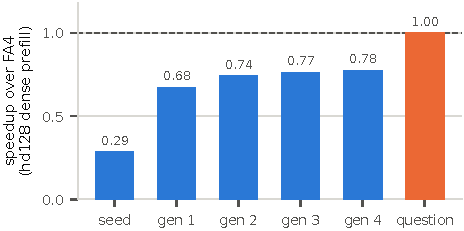
\includegraphics[width=\columnwidth]{figures/evo.pdf}
\caption{Evolutionary search on the Blackwell dense-prefill kernel, then one question. Four
generations of an AVO-style loop (six mutations each, monotone lineage, a strategist writing
hypothesis-shaped directives) took a correct port from 0.29$\times$ to 0.78$\times$ of FA4. The
remaining gap was outside the kernel: a question about where the time was going located a
synchronous host copy of about 38~$\mu$s per call, and removing it brought the dense envelope to
parity.}
\label{fig:evo}
\end{figure}

\begin{figure}[t]
\centering
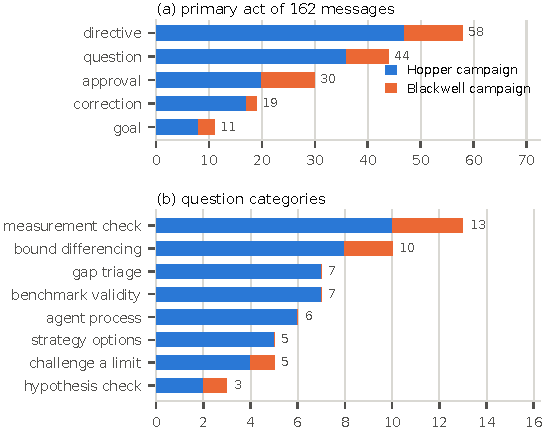
\includegraphics[width=\columnwidth]{figures/messages.pdf}
\caption{The 162 human messages across the 16 \sys sessions. (a) Primary act. (b) Categories of
the 56 messages whose primary act was a question, excluding 8 housekeeping questions about the
repository.}
\label{fig:messages}
\end{figure}

\paragraph{Sources.} Sixteen \sys sessions are archived: nine Claude Code sessions as JSONL
transcripts with their subagent transcripts, and seven Cursor sessions as exported JSONL. Claude
Code transcripts record the model per assistant message (\texttt{claude-opus-4-8} in seven sessions,
\texttt{claude-opus-5} in two); Cursor exports do not. The equipped agent's run is a checkpoint
directory with one record per candidate (source, build, correctness, timing, promotion decision,
timestamp) and the orchestrator's log, memory file, and knowledge store.

\paragraph{Parsing.} A tool call is an assistant content block of type tool use, de-duplicated by
its identifier across the parent transcript and any compaction summaries; a subagent's calls are
counted separately and attributed to the parent session. Human turns are user messages that are not
tool results, Stop-hook injections, or system reminders; in Cursor exports they are identified by
the user record's timestamp tag. Tool calls are classified by regular expressions over the tool
name and arguments into: profiler runs, SASS or PTX inspections, builds, benchmark or evaluator runs,
documentation reads, sanitizer runs, and reads of the agent's own kernel files; the categories
overlap where a shell command does two things. The ``tool-result text re-reading own kernel'' figure
of Table~\ref{tab:h2h} is the share of tool-result characters returned by file reads whose path is
one of the kernel sources, over all tool-result characters in the Claude Code parent transcripts
(26\%; for the equipped agent, the same quantity over its per-step tool logs, 82\%).

\paragraph{Labeling.} One author labeled each of the 162 human messages by its primary act (goal,
directive, question, approval, correction), flagged whether it was phrased as a question, and
assigned the 44 question-act messages and the 12 question-shaped corrections to the categories of
\S\ref{sec:workflow-questions}; eight further questions concerned repository housekeeping and are
excluded from Figure~\ref{fig:messages}(b). The agent-side counts (35 structured questions to the
human, 24 offering to accept or stop, 126 limit assertions, 59 Stop-hook returns) are from the Claude
Code sessions only, where these events are structured; the Cursor exports do not separate them.
Figure~\ref{fig:messages} shows the resulting distribution. The labels, the parsing scripts, and the
per-session inventory are released with the traces.

\section{Baseline Agent Details}
\label{app:baseline}

\begin{table}[t]
\centering\small
\caption{What \baseline supplied to the model at every step.}
\label{tab:baseline}
\setlength{\tabcolsep}{4pt}
\begin{tabular}{@{}p{0.34\columnwidth}p{0.6\columnwidth}@{}}
\toprule
Component & Distilled output in the prompt \\
\midrule
Lever selector & one of 16 optimizations, keyed to the NCU bottleneck label \\
NCU parser & bottleneck diagnosis for the worst configuration \\
SASS analyzer & instruction-mix deltas vs.\ the champion and a CUTLASS oracle \\
Doc retrieval & BM25 over the PTX ISA, CUDA guide, NCU and Nsight docs, CUTLASS docs, Hopper tuning guide \\
Reference libraries & hints extracted from DeepGEMM, ThunderKittens, CUTLASS (1.6~GB on disk) \\
Knowledge store & typed notes (kernel, profiling, algorithmic), 15 seeded \\
Memory & causal lessons from recent steps: change, hypothesis, outcome, cause \\
Sanitizer, anti-cheat & bounded compute-sanitizer runs; forbidden-symbol checks \\
\bottomrule
\end{tabular}
\end{table}

Table~\ref{tab:baseline} lists the components of \baseline and what each contributed to the step
prompt. The per-step prompt assembled, in order: the task statement and hard rules; the chosen lever
with its rationale; the NCU diagnosis for the worst configuration; the SASS instruction-mix deltas
against the champion; the retrieved documentation sections; the reference-library hints; the
knowledge-store notes matching the lever; the memory file's recent lessons; the current champion
source; and the instruction to write one improved candidate to a fixed path and stop. The median
prompt was 22.6K characters excluding the champion source, 37\% of it retrieved or pre-fetched
material. Promotion required a correct candidate whose worst-configuration ratio exceeded the
champion's by more than a 3\% noise band. The plateau detector fired after eight steps without
promotion and opened a rewrite branch seeded at the lineage's pre-plateau knee; 37 branches were
opened, 36 from the same step. Three human rollbacks discarded 117 steps. The run's 313 kept steps,
the 133 model-driven ones among them, the memory file, and the knowledge store are released with
the specification from which the agent was built.

\section{Benchmark Methodology}
\label{app:bench}

\paragraph{Timing.} Each scenario is timed on one GPU with every implementation run back to back
from byte-identical inputs. After 20 warm-up calls, the harness takes three trials of 40 CUDA-event
samples each, flushing a 32~MB buffer through L2 and synchronizing before every sample, and reports
the median of the 120 samples; the per-scenario speedup is the upstream median over the
implementation's median. Clocks are not locked, which is why only ratios are reported. cuDNN and
FlashInfer are given the same packed and paged buffers as our kernel and the upstream, and a
scenario is marked unsupported for an implementation when it rejects the configuration or fails
correctness.

\paragraph{Correctness.} Every candidate's outputs are compared with the upstream kernel's and with
an fp32 reference on every scenario, with a per-dtype tolerance; a candidate that fails any scenario
scores zero. In the head-to-head, the equipped agent's gate additionally required token-for-token
equality with FA3 on a greedy decode inside vLLM.

\paragraph{Repeats and noise.} The Hopper suite was run as three full repeats in each of four
independent batches on the 8$\times$H200 node, one scenario per GPU at a time, with a single-GPU
serial control that agrees with the parallel runs to within 0.8\%. Per-scenario medians over the
three repeats are the reported numbers; the four batches agree to within 0.3\% on every aggregate,
and per-scenario ratios vary by 1\% at the median and 6\% at most. The Blackwell suite was run once
on the 8$\times$B200 node with the same protocol. The \texttt{edge} scenarios are short kernels for
which dispatch overhead is a visible share of wall-clock time, so their ratios overstate kernel-only
gains; the \texttt{claim} and \texttt{real} sets are long enough that dispatch is negligible.
